% IF YOU CAN SEE THIS GO CONTRIBUTE >:(

\documentclass[letterpaper, 8pt]{extarticle}
\usepackage{amssymb,amsmath,amsthm,amsfonts}
\usepackage{multicol,multirow}
\usepackage{calc}
\usepackage{ifthen}
\usepackage[landscape]{geometry}
\usepackage[colorlinks=true,citecolor=blue,linkcolor=blue]{hyperref}

\usepackage{booktabs}
\usepackage{ulem}
\usepackage{enumitem}
\usepackage{tabulary}
\usepackage{graphicx}
\usepackage{siunitx}
\usepackage{tikz}
\usepackage{derivative}
\usepackage{svg}
\usepackage{listings}
\usepackage{setspace}
\usepackage{listings}
\usepackage{xcolor}
\usepackage{courier}

% minimal line spacing
\setstretch{0.1}

% set borders (experimentally determined to minimize cutoff and maximize space on school printers)
\geometry{top=.25in,left=.25in,right=.25in,bottom=.35in}

% make figures work better in multicol
\newenvironment{Figure}
{\par\medskip\noindent\minipage}
{\endminipage\par\medskip}

\pagestyle{empty} % clear page

% rewrite section commands to be smaller
\makeatletter
\renewcommand{\section}{\@startsection{section}{1}{0mm}%
                                {-1explus -.5ex minus -.2ex}%
                                {0.5ex plus .2ex}%x
                                {\normalfont\normalsize\bfseries}}
\renewcommand{\subsection}{\@startsection{subsection}{2}{0mm}%
                                {-1explus -.5ex minus -.2ex}%
                                {0.5ex plus .2ex}%
                                {\normalfont\small\bfseries}}
\renewcommand{\subsubsection}{\@startsection{subsubsection}{3}{0mm}%
                                {-1ex plus -.5ex minus -.2ex}%
                                {1ex plus .2ex}%
                                {\normalfont\tiny\bfseries}}
\makeatother
\setcounter{secnumdepth}{0} % disable section numbering

% disable indenting
\setlength{\parindent}{0pt}
\setlength{\parskip}{0pt plus 0.5ex}

% Custom siunitx defs
\DeclareSIUnit\noop{\relax}
\NewDocumentCommand\prefixvalue{m}{%
\qty[prefix-mode=extract-exponent,print-unity-mantissa=false]{1}{#1\noop}
}

% Shorthand definitions
\newcommand{\To}{\Rightarrow}
% holy fck thanks for this
\newcommand{\ttt}{\texttt}

% condense itemize & enumerate
\let\olditemize=\itemize \let\endolditemize=\enditemize \renewenvironment{itemize}{\olditemize \itemsep0em}{\endolditemize}
\let\oldenumerate=\enumerate \let\endoldenumerate=\endenumerate \renewenvironment{enumerate}{\oldenumerate \itemsep0em}{\endoldenumerate}
\setlist[itemize]{noitemsep, topsep=0pt, leftmargin=*}
\setlist[enumerate]{noitemsep, topsep=0pt, leftmargin=*}

\title{3SH3}

\begin{document}
% \raggedright
\tiny

% make listings look nicer
\lstset{
    tabsize = 2, %% set tab space width
    showstringspaces = false, %% prevent space marking in strings, string is defined as the text that is generally printed directly to the console
    basicstyle = \tiny\ttfamily, %% set listing font and size
    breaklines = true, %% enable line breaking
    numberstyle = \tiny,
    postbreak = \mbox{\textcolor{red}{\(\hookrightarrow\)}\space}
}

\begin{center}
    {\textbf{3SH3 Final -- Linus Torvalds Edition}} \\
\end{center}
% set column spacing rules
\setlength{\premulticols}{1pt}
\setlength{\postmulticols}{1pt}
\setlength{\multicolsep}{1pt}
\setlength{\columnsep}{2pt}
\begin{multicols*}{6}
    % sections based on slide titles
    \section{Overview}
    \textbf{System Programs:} associated with the operating system but are not
    necessarily part of the kernel.\\
    \textbf{Middleware:} software frameworks that provide additional services to
    application developers.

    \subsection{Interrupts}
    Signal to CPU there is a task requiring attention, usually I/O. Trap is s/w generated interrupt caused by error or user request. \\
    \textbf{Synchronous:} user process waits for I/O to finish, must know time it takes. \textbf{Asynchronous:} request returns before I/O completion, interrupts when done. \\
    \textbf{Polling system:} system calls all interrupt handlers to determine which made the interrupt. (slow) \textbf{vectored system:} handler is found via interrupt vector. \\
    Interrupt is \underline{maskable} if it can be ignored by CPU otherwise \underline{nonmaskable}.

    \subsection{I/O Techniques}
    \textbf{Programmed:} Requested I/O action performed, module sets I/O status register. Processor periodically checks status until action completed. \\
    \textbf{Interrupt-driven:} Process issues I/O command to module which interrupts processor when done. Processor then transfers data. \\
    \textbf{DMA:} Data is transferred directly to memory, processor only needed for initialization. Bus access slowed for processor during the transfer.

    \section{Processes}
    \textbf{Possible states of a process}: new, running, waiting, ready,
    terminated.
    \subsection{Process Creation Code}
    \begin{lstlisting}[language=C]
int main()
{
    pid_t pid;
    /* fork a child process */
    pid = fork();
    if (pid < 0) { /* error occurred */
        fprintf(stderr, "Fork Failed");
        return 1;
    }
    else if (pid == 0) { /* child process */
        execlp("/bin/ls","ls",NULL);
    }
    else { /* parent process */
        /* parent will wait for the child to complete */
        wait(NULL);
        printf("Child Complete");
    }
    return 0;
}
\end{lstlisting}
    \ttt{Fork()} returns 0 for the child process, and returns the \ttt{pid} of the 
    child process for the parent.
    The \ttt{exit(1)} system call can be used to terminate a process with
    status 1. The parent can obtain the status of a terminated child with
    \ttt{pid = wait(\&status)} where \ttt{status} is the integer status of the
    child process.
    A process that has terminated, but whose parent has not yet called \verb|wait()|,
    is a \textbf{zombie} process.
    If the parent of a process terminated without invoking \verb|wait()|,
    the process is an \textbf{orphan}.

    \subsection{Posix Shared Memory}
    \begin{lstlisting}[language=C]
/* create the shared memory object */
fd = shm open(name,O_CREAT | O_RDWR,0666);
/* configure the size of the shared memory object */
ftruncate(fd, SIZE);
/* memory map the shared memory object */
ptr = (char *)
mmap(0, SIZE, PROT_READ | PROT_WRITE, MAP_SHARED, fd, 0);

/* write to the shared memory object */
sprintf(ptr,"%s",message_0);
ptr += strlen(message_0);
sprintf(ptr,"%s",message_1);
ptr += strlen(message_1);
/* read from the shared memory object */
printf("%s",(char *)ptr);

/* remove the shared memory object */
shm_unlink(name);
\end{lstlisting}

    \subsection{Pipes (message passing)}
    \begin{lstlisting}[language=C]
#define BUFFER_SIZE 25
#define READ_END 0
#define WRITE_END 1
int main(void)
{
    char write_msg[BUFFER_SIZE] = "Greetings";
    char read_msg[BUFFER_SIZE];
    int fd[2];
    /* create the pipe */
    if (pipe(fd) == -1) {
        fprintf(stderr,"Pipe failed");
        return 1;
    }
    /* fork a child process */
    pid = fork();
    if (pid < 0) { /* error occurred */
        fprintf(stderr, "Fork Failed");
        return 1;
    }
    if (pid > 0) { /* parent process */
        /* close unused end of pipe */
        close(fd[READ_END]);
        /* write to pipe */
        write(fd[WRITE_END], write msg, strlen(write msg)+1);
        /* close write end of pipe */
        close(fd[WRITE_END]);
    }
    else { /* child process */
        /* close unused end of pipe */
        close(fd[WRITE_END]);
        /* read from pipe */
        read(fd[READ_END], read msg, BUFFER SIZE);
        printf("read %s",read msg);
        /* close read end of pipe */
        close(fd[READ_END]);
    }
    return 0;
}
\end{lstlisting}
    \section{Threads}
    \subsection{Amdahl's Law}
    $speedup \leq \frac{1}{S+(1-S)/N}$ where $S$ is the serial
    portion of the application and $N$ is the number of processing cores

    \textbf{Threads of a process share} the code section, data section, and files
    of the process. The registers, stack, and program counter of the threads
    differ.

    \textbf{Data Parallelism:} distribute subsets of the same data across multiple
    computing cores. \\
    \textbf{Task Parallelism:} distribute tasks (threads) across multiple
    computing cores.

    \textbf{Five areas of challenge in multicore programming:} identifying tasks,
    balancing the amount of work tasks do, data splitting, data dependency,
    and testing and debugging.

    \textbf{Synchronous Signals:} Delivered to the same process that caused the
    signal.
    \textbf{Asynchronous Signals:} Delivered to a process that did not cause the
    signal.

    \textbf{Thread Local Storage (TLS):} Data local to a specific thread. Similar
    to the concept of static data and local variables.

    \textbf{Lightweight Processes (LWP):} Intermediate data structure between
    user and kernel threads often used in systems implementing many-to-many or
    two-level thread models. Looks like a virtual processor to the user-thread
    library. The application can schedule a user thread to
    run on an LWP. Each LWP is attached to a kernel thread, and it is kernel
    threads that the operating system schedules to run on physical processors.
    If a kernel thread blocks, the LWP blocks and also blocks the user thread
    down the chain.

    \textbf{Benefits of Threads:} \underline{Responsiveness},
    \underline{resource sharing} (threads share data by default),
    \underline{economy} (threads are take less time and memory to create
    threads then processes), \underline{scalability}.
    \subsection{Pthread}
    \begin{lstlisting}[language=C]
pthread_t tid; /* thread identifier */
pthread_attr t attr; /* set of thread attributes */
/* set default attributes of thread */
pthread_attr_init(&attr);
/* create the thread */
pthread_create(&tid, &attr, runner, argv[1]);
/* cancel the thread */
pthread_cancel(tid);
/* check if there is a cancellation request */
pthread_testcancel();
/* wait for the thread to exit */
pthread_join(tid,NULL);
pthread_exit(0);
\end{lstlisting}
    \section{Synchronization}
    \subsection{Critical section problem}
    A solution to the critical section problem must satisfy
    \underline{mutual exclusion},
    \underline{progress} (processes are eventually allowed to access their
    critical sections after requesting it), and
    \underline{bounded} waiting (there is a limit
    on the number of times other processes can access their critical sections
    after one process has requested access)
    \textbf{Peterson's Solution:} processes use a flag variable to indicate
    if a process is ready to enter its critical section and a shared
    turn variable to indicate which process' turn it is to enter their
    critical section.


    \subsection{Semaphores}
    \texttt{wait()} = \texttt{P()}, \texttt{signal()} = \texttt{V()},
    \texttt{wait()} decrements the semaphore, \texttt{signal()} increments the
    semaphore.

    \subsection{Atomic Instructions}
    \begin{lstlisting}[language=C]
boolean test_and_set(boolean *target) {
    boolean rv = *target;
    *target = true;
    return rv;
}
do {
    while (test_and_set(&lock))
        ; /* do nothing */
        /* critical section */
    lock = false;
        /* remainder section */
} while (true);

int compare_and_swap(int *value, int expected, int new_value) {
    int temp = *value;
    if (*value == expected)
        *value = new_value;
    return temp;
}
while (true) {
    while (compare_and_swap(&lock, 0, 1) != 0)
        ; /* do nothing */
        /* critical section */
    lock = 0;
        /* remainder section */
}
\end{lstlisting}

    \textbf{Liveness:} A set of properties that a system must satisfy to ensure
    that processes make progress during their execution life cycle.

    \subsection{Pthread Synchronization}

    \subsubsection{Mutex Locks}
    \begin{lstlisting}[language=C]
pthread_mutex_t mutex;
/* create and initialize mutex lock */
pthread_mutex_init(&mutex,NULL);
/* acquire the mutex lock */
pthread_mutex_lock(&mutex);
/* critical section */
/* release the mutex lock */
pthread_mutex_unlock(&mutex);
    \end{lstlisting}

    \subsubsection{Condition Variables}
    \begin{lstlisting}[language=C]
pthread_mutex_t mutex;
pthread_cond_t cond_var;

pthread_mutex_init(&mutex,NULL);
pthread_cond_init(&cond_var,NULL);

// thread waiting on condition variable
pthread_mutex_lock(&mutex);
while (a != b)
    pthread_cond_wait(&cond_var, &mutex);

pthread_mutex_unlock(&mutex);

// thread that modifies shared data, signalling waiting thread
pthread_mutex_lock(&mutex);
a = b;
pthread_cond_signal(&cond_var);
pthread_mutex_unlock(&mutex);
\end{lstlisting}
    \section{Deadlocks}
    % If someone thinks of a better subsection name just change it.
    \subsection{Is Deadlock Possible}
    % TODO: #14 Rewrite deadlock info as not a question
    % Assume that a multithreaded application uses only reader-writer locks for synchronization. Applying the four necessary conditions for dead-lock, is deadlock still possible if multiple reader-writer locks are used?\\
    % Answer: Yes.\\
    % (1) Mutual exclusion is maintained, as locks cannot be shared if there is a writer.\\
    % (2) Hold and wait is possible, as a thread can hold one reader-writer lock while waiting to acquire another.\\
    % (3) You cannot take a lock away, so no preemption is upheld.\\
    % (4) A circular wait among all threads is possible.\\
    \subsubsection{Necessary Conditions}
    \textbf{Mutual Exclusion} - A resource can only be held by one process at a time.
    \textbf{Hold and Wait} - A process can hold a number of resources at a time and at the same time,
    it can request for other resources that are being held by some other process.
    \textbf{No preemption} - A resource can't be preempted from the process by another process, forcefully.
    \textbf{Circular Wait} - There is a circular dependency of resources that processes are waiting for.
    \subsubsection{Reader-writer locks}
    If only reader-writer locks are used in a multithreaded application, then deadlock is still possible.\\
    Locks cannot be shared if there is a writer(mutual exclusion).\\
    A thread can hold one reader-writer lock while waiting to acquire another(hold and wait).\\
    You cannot take a lock away, so no preemption is upheld.\\
    A circular wait among all threads is possible.
    \subsection{Banker's Algorithm}
    Need = Max - Allocation.\\
    Safe state = all threads can finish executing with the available resources.\\
    If need $<$ available for a particular resource for all (remaining) threads then not in safe state. \\
    Otherwise execute the threads that can be executed until no threads remain.

    \subsection{Resource Allocation Graphs}
    A directed edge from thread $T_i$ to resource type $R_j$ is denoted
    by $T_i \rightarrow R_j$; and signifies that thread $T_i$ has requested
    an instance of resource type $R_j$. \\
    A directed edge from resource type $R_j$ to thread $T_i$ is denoted by
    $R_j \rightarrow T_i$ signifies that an instance of resource type
    $R_j$ has been allocated to thread $T_i$.

    \subsection{Methods for Handling Deadlock}
    \textbf{Deadlock Prevention:} prevent circular wait from happening
    (only practical solution) \\
    \textbf{Deadlock Avoidance:} don't grant resources if it leads the
    system to an unsafe state.\\
    \textbf{Deadlock Detection and Recovery:} Either terminate or preempt
    resources.
    \section{Scheduling}

    \subsection{Predicting next CPU burst Formula}
    $\tau_{n+1} = \alpha \cdot t_n + (1-\alpha) \cdot \tau_n$
    where $t_n$ is the value of the nth CPU burst, $0 \leq \alpha \leq 1$ \\
    $\tau_0$ affects the starting value of the predictions,
    and $\alpha$ affects how much the last CPU burst vs
    the last predicted CPU burst is weighted.\\
    If $\alpha = 0$, then $\tau_{n+1} = \tau_n$ and recent history has
    no effect on the future CPU burst. If $\alpha = 1$, then
    $\tau_{n+1} = t_n$ and only the most recent CPU bursts matter (history
    is assumed to be old and irrelevant). $\alpha = 1/2$ weights recent
    and past history evenly.
    \subsection{Scheduling Algorithms Formulas}
    \textbf{Throughput:} Number of processes completed per time unit
    \textbf{Turnaround time of a process} is difference between when
    the process finishes execution and its arrival time;
    turnaround time = process finish time - start time.
    \textbf{Waiting time of a process} is how long a process does not execute
    on the CPU from its arrival. The time a process spends waiting on the
    ready queue.
    \textbf{CPU utilization rate} is the time the CPU spends executing
    processes divided by the total time (time spent executing + time spent idle)
    \textbf{Response Time:} The difference between the time a process
    produces a response and the time of the submission of a request
    (possibly same as arrival time?)

    \textbf{SJF} cannot be implemented at the level of CPU scheduling because
    you cannot know the length of the next CPU burst (you can't see the future).

    For \textbf{round robin scheduling}, the time quantum should be large
    with respect to the context switch time so not too many context switches
    are done, but not too large so as to devolve to FCFS scheduling.

    \subsection{Chip Multithreading}
    When you have more than one hardware thread in a core. The threads look
    like two logical CPUs to the OS. 

    \textbf{Coarse grained multithreading:} a thread executes on a core until a
    long-latency event such as a memory stall occurs. Because of the delay
    caused by the long-latency event, the core must switch to another thread to
    begin execution. However, the cost of switching between threads is high,
    since the instruction pipeline must be flushed before the other thread can
    begin execution on the processor core.\\
    \textbf{Fine grained multithreading:} threads switch at the boundary of
    an instruction cycle. Fine-grained systems include logic
    for thread switching, so the cost of switching between threads is small.

    \subsection{Load Balancing}
    \textbf{Push migration:} a specific task periodically checks the
    load on each processor and if it finds an an overloaded processor it
    evenly distributes the load by pushing/moving threads to idle or less-busy
    processors.\\
    \textbf{Pull migration:} when an idle processor pulls a waiting task
    from a busy processor.

    \subsection{Processor Affinity}
    A process has an ``affinity'' for the processor it is currently
    running on because the process will usually have values it uses often
    in the cache of the current processor.\\
    \textbf{Soft Affinity:} OS will attempt to keep a process on a single
    processor, but it is possible for a process to migrate
    between processors during load balancing.
    \textbf{Hard Affinity:} OS allows a process to specify a subset of
    processors on which it can run using sys calls.

    \subsection{Real time Scheduling}
    The scheduler for a real-time operating system must support a priority based
    algorithm with preemption

    \textbf{Event latency:} amount of time that elapses from when an event occurs
    to when it is serviced.\\
    \textbf{Interrupt latency} refers to the period of time from the arrival of
    an interrupt at the CPU to the start of the routine that services the
    interrupt.\\
    \textbf{Dispatch latency} amount of time required for the scheduling
    dispatcher to stop one process and start another.

    \textbf{Little's Formula:} $n = \lambda \cdot W$ where $n$ is the
    average long-term queue length (excluding the process being serviced),
    $\lambda$ is the average arrival rate for new processes in the queue,
    and $W$ is average long-term queue length.

    \subsection{Gantt Chart}
    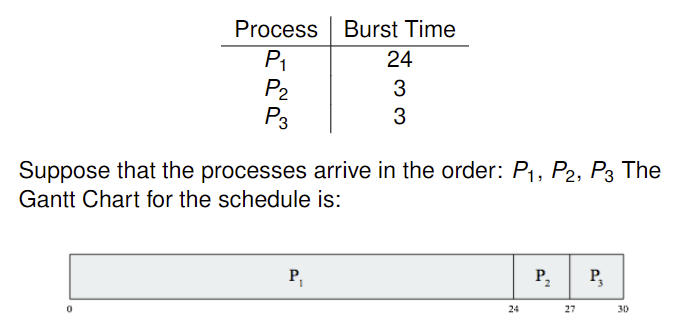
\includegraphics[width=\linewidth]{gantt-chart.png}

    \section{Memory Management}

    \textbf{Dynamic loading:} a routine is not loaded until it is called. All
    routines are kept on disk in a relocatable load format. The main program is
    loaded into memory and is executed. When a routine needs to call another
    routine, the relocatable linking loader is called to load
    the desired routine into memory if its not loaded and
    to update the program’s address tables to reflect this change. Then control is
    passed to the newly loaded routine.\\
    \textbf{Dynamic Linked Libraries} are similar.

    \subsection{Fragmentation}
    \textbf{First fit} strategy given N blocks will lose 0.5N blocks to
    fragmentation; 1/3 of memory will be unusable. Is also called the
    50\% rule. \\
    \textbf{Compaction} is only possible if relocation is dynamic and
    done at runtime, not possible if relocation is static and done at
    assembly or load time.

    \subsection{Paging}
    If the size of the logical address space is 2m, and a
    page size is 2n bytes, then the high-order m-n bits of a logical address
    designate the page number, and the n low-order bits designate the page
    offset.\\
    If process size is independent of page size, we expect internal fragmentation
    to average one-half page per process.\\
    The \textbf{frame table} has one entry for each physical page frame,
    indicating whether the latter is free or allocated and, if it is allocated,
    to which page of which process (or processes). Used by the OS to keep
    track of physical memory.\\
    \textbf{Reentrant code} is non-self-modifying code: it
    never changes during execution and can be shared among processes. Can be
    implemted as shared pages.\\

    \subsubsection{Number of Bits and/or Entries}
    \textbf{Important}: if any size is not in bytes convert to bytes first.\\
    If the address takes \(x\) bits to store,
    page size is $2^y$ bytes,
    and number of frames or pages is $2^z$,
    then $x = y + z$.\\
    If there are $2^x$ amount of pages/frames and the page size is $2^y$, then the logical/physical address is $x+y$ bits long. \\
    \textbf{Conventional single level} page table stores an entry for each virtual page or page number.
    \textbf{Inverted page table} stores an entry for each physical frame.

    % NOTE: remove me if we run out of space
    \subsubsection{Internal Fragmentation Formula}
    Given page size = \(p\), process size \(r\), pages used = \(n\),
    \(\textrm{fragmentation} = n \cdot p - r\)

    \section{Virtual Memory}
    \subsection{Demand Paging}
    $\text{\textbf{effective access time}} = (1-p) \cdot ma + p \cdot \text
        {page fault time}$ where $p$ is the probability of a page fault and $ma$
    is the memory access time.\\
    A \textbf{valid/invalid bit} is used to tell a process if a page is legal
    and in memory or if its invalid (not in address space of the process) or
    legal but not in memory.\\
    OS' maintain a \textbf{free frames list} which is a pool of free frames for
    satisfying requests for new pages being brought into memory.\\
    \textbf{Zero-fill-on-demand:} the contents of frames are erased before
    being allocated.\\

    \section{File System}

    \textbf{Volume:} disk block that contains file system.\\

    \textbf{Info associated with an open file:} file pointer, file-open count,
    location of the file, and access rights to the file.\\

    \textbf{Operations to be performed on a directory:} search for a file,
    create a file, delete a file, list a directory, rename a file, traverse
    the file system.

    \subsection{Directory Structure}
    \textbf{Single-level directory:} Only one directory exists for all
    users and all files are kept in it.\\
    \textbf{Two-level directory:} Each user has their own directory and a
    master file directory is indexed by username to point to the user's
    directory. Isolates users from each other. Is a tree of height 2. \\
    \textbf{Garbage collection} involves traversing the entire file
    system, marking everything that can be accessed. Then, a second pass
    collects everything that is not marked onto a list of free space.
    Only used in general graph directory structures.

    \textbf{Logic for ``answering maximum size of file'' type questions}: multiply the
    number of direct disk blocks by size of the disk blocks, for indirect
    disk blocks, divide the size of the disk blocks by the size of a pointer to
    a disk block, then raise this number by a power which is the same as the
    level of the indirect block (i.e. for single indirect raise by a power of
    1, for a double indirect raise by a power of 2, and so on).
    Multiply this value
    by the size of a disk block and by the amount of that specific indirect
    disk block, i.e. if you are doing the calculation for 5 single indirect
    disk blocks, then multiply by 5 at the end. Add the multiplications
    for all the types of disk blocks together for the final answer.

    \section{Mass Storage Systems}
    \subsection{SCAN Scheduling}
    The disk arm starts at one end of the disk and moves
    toward the other end, servicing requests as it reaches each cylinder,
    until it gets to the other end of the disk. At the other end, the
    direction of head movement is reversed, and servicing continues
    \subsection{C-SCAN Scheduling}
    C-SCAN moves the head from one end of
    the disk to the other, servicing requests along the way. When the
    head reaches the other end, however, it immediately returns
    to the beginning of the disk without servicing any requests on the
    return trip. Is a variant of SCAN scheduling.

    \textbf{Write amplification:} The creation of I/O requests not by applications
    but by the NVM device doing garbage collection and space management. Can
    greatly impact the write performance of the device.
    \subsection{latency \& I/O time}
    Latency based on spindle speed: 1/ (RPM/60) = 60/RPM\\
    Average latency = 1/2 latency\\
    Access Latency = average seek time + average latency\\
    Average I/O time = access latency + (amount to transfer / transfer rate) + controller overhead

    \section{Conversions}
    \qty{1}{\second} = \qty{1000}{\milli\second},
    \qty{1}{\milli\second} = \qty{1000}{\micro\second} (microsecond),
    \qty{1}{\micro\second} = \qty{1000}{\nano\second}

    \qty{1}{\kilo\byte} = \qty[parse-numbers=false]{2^{10}}{\byte} = 1024 B,\\
    \qty{1}{\mega\byte} = \qty[parse-numbers=false]{2^{20}}{\byte} = 1,048,576 B,\\
    \qty{1}{\giga\byte} = \qty[parse-numbers=false]{2^{30}}{\byte} = 1,073,741,824 B,\\
    \qty{1}{\tera\byte} = \qty[parse-numbers=false]{2^{40}}{\byte} = 1,099,511,627,776 B

\end{multicols*}
\end{document}
